\section{Marco teorico} 
¿Qué es un ORM?
\begin{itemize}
	\item El Mapeo Objeto-Relacional o ORM  es un modelo de programacion que consiste en la transformar la logica de programacion (entidades) en tablas, simplificando las tareas como son el modelado.
	\\La ventaja mas certeras en el ORM es la capacidad de poder migrar la DB sin la necesidad de saber todo el entorno completo ya que se trabajaria con un lenguaje unificado.
	\begin{center}
	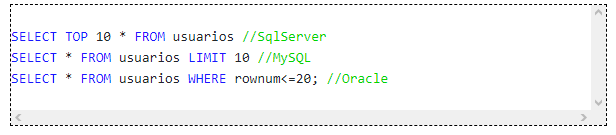
\includegraphics[width=13cm]{./Imagenes/orm_1} 
	\end{center}
	Mismo proposito diferentes formas de hacerlo.
	\begin{center}
	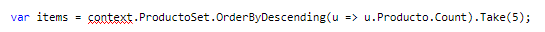
\includegraphics[width=13cm]{./Imagenes/orm_2} 
	\end{center}
	En este caso la anterior linea de codigo tiene el mismo proposito que la primera imagen.

\end{itemize} 